\documentclass[a4paper]{report}

\usepackage{graphicx}
\usepackage{float}
\usepackage{hyperref}
\usepackage[spanish]{babel}

\begin{document}

\title{Universidad Nacional de La Plata\\Facultad de Inform\'atica\\ \bigskip
  Especializaci\'on en C\'omputo de Altas Prestaciones\\ \bigskip
  Herramientas para el Soporte de An\'alisis de Rendimiento}

\author{
  Alumno: Andr\'es More - {\tt amore@hal.famaf.unc.edu.ar}\\
  Director: Dr Fernando G. Tinetti - {\tt fernando@lidi.info.unlp.edu.ar}
}

%\date{}

\maketitle

\begin{abstract}

  Este documento describe una investigaci\'on realizada como trabajo final para
  la Especializaci\'on en C\'omputo de Altas Prestaciones dictada en la
  Facultad de Inform\'atica de la Universidad Nacional de La Plata.
  El tema de investigaci\'on consiste en m\'etodos y herramientas para
  el an\'alisis del comportamiento de aplicaciones de alto rendimiento.

  \bigskip

  Luego de la introducci\'on de terminolog\'ia y bases te\'oricas del
  an\'alisis cuantitativo de rendimiento, se resume la experiencia de utilizar
  herramientas para conocer donde se deber\'ia localizar los esfuerzos de
  optimizaci\'on. Antes de concluir se propone un modelo para este tipo de
  aplicaciones utilizando una abstracci\'on en etapas, cuya
  utilizaci\'on simplifica el an\'alisis de rendimiento y facilita el proceso de optimizaci\'on.

  \bigskip

  Este trabajo resume la experiencia que debe atravesar cualquier
  individuo en busca de las diferentes alternativas para el an\'alisis de
  rendimiento; incluyendo la selecci\'on de herramientas de soporte y la
  definici\'on de un procedimiento rudimentario para la aplicaci\'on sistem\'atica
  de las mismas.

  \bigskip

  Este trabajo contribuye entonces con un resumen de las teor\'ia del an\'alisis del
  rendimiento m\'as una descripci\'on de los herramientas de soporte 
  disponibles actualmente. Se propone tambi\'en un proceso para analizar el
  rendimiento, ejemplificando su aplicaci\'on a un conjunto de n\'ucleos de
  c\'omputo no triviales.

\end{abstract}

\tableofcontents

\chapter{Introducci\'on}

Este cap\'itulo introduce este trabajo y su alcance. Luego de revisar la
motivaci\'on de esta investigaci\'on, se resume el estado actual del an\'alisis
del rendimiento y se detalla el contenido restante del informe.

\section{Motivaci\'on}

En el \'area de c\'omputo de altas prestaciones los desarrolladores son los mismos
especialistas del dominio del problema a resolver. Las rutinas
m\'as demandantes de c\'alculo son en su mayor\'ia cient\'ificas y su
alta complejidad hace posible su correcta implementaci\'on s\'{o}lo por los mismos investigadores.
Este hecho resulta en un reducido tiempo de an\'alisis de resultados
e impacta directamente en la productividad de cualquier grupo de investigaci\'on.

\bigskip

Con mayor impacto que en otras \'areas de la computaci\'on, el c\'odigo
optimizado correctamente puede ejecutarse \'ordenes de magnitud mejor que una implementaci\'on
directa \cite{mm-matrixmultiplicationtool}. Adem\'as, se utiliza
programaci\'on en paralelo para obtener una mejor utilizaci\'on de la
capacidad de c\'omputo disponible; aumentando la complejidad de implementaci\'on, depuraci\'on y
optimizaci\'on \cite{parallel-programming}.

\bigskip

El proceso de optimizaci\'on de una implementaci\'on termina entonces siendo
hecho de modo {\it ad-hoc}, sin conocimiento pleno de las herramientas disponibles y
sus capacidades, y sin la utilizaci\'on de informaci\'on cuantitativa para dirigir los
esfuerzos de optimizaci\'on. Es frecuente la implementaci\'on directa
de algoritmos en lugar de la utilizaci\'on de librer\'ias ya disponibles, optimizadas
profundamente y con correctitud comprobada por el paso del tiempo.

\section{Alcance}

Este trabajo considera en particular a los sistemas de memoria distribu\'ida corriendo sobre
GNU/Linux, denominados sistemas Beowulf \cite{beowulf}. A trav\'es de las
estad\'isticas mostradas por el Top500 \footnote{El Top500 es una lista actualizada de supercomputadoras
de acuerdo al benchmark Linpack, disponible en {\tt http://www.top500.org}.}, se
puede determinar que son los m\'as utilizados en el c\'omputo de aplicaciones de alto rendimiento.

\section{Estado Actual}

Actualmente existen diversas herramientas para el an\'alisis de rendimiento.
Estas funcionan a diferentes niveles de abstracci\'on: desde contadores de eventos
a nivel de {\it hardware}, pasando por soporte del n\'ucleo del sistema operativo para ofrecer
monitores del uso de los recursos disponibles, hasta la
simple utilizaci\'on del tiempo de ejecuci\'on de una aplicaci\'on o la comparaci\'on contra un trabajo de referencia.

\section{Organizaci\'on del Contenido}

El resto del documento explica inicialmente teor\'ia sobre el an\'alisis del rendimiento, que luego es
aplicada a trav\'es de diversas herramientas.

\bigskip

El cap\'itulo 2 discute el an\'alisis de rendimiento, sus
principios y teor\'ia. El cap\'itulo 3 detalla las herramientas m\'as
utilizadas. El cap\'itulo 4 ejemplifica la aplicaci\'on de las herramientas
para obtener informaci\'on de an\'alisis a trav\'es de un proceso sistem\'atico.
El cap\'itulo 5 concluye y el cap\'itulo 6 detalla posibles trabajos futuros o extensiones a considerar.

\chapter{An\'alisis de Rendimiento}

Este cap\'itulo introduce el concepto de rendimiento y teor\'ia b\'asica sobre su an\'alisis.

\section{Definici\'on}

El rendimiento se caracteriza por la cantidad de trabajo de c\'omputo que se
logra en comparaci\'on con la cantidad de tiempo y el uso de los recursos  empleados.
El rendimiento es evaluado entonces de forma cuantificable, utilizando alguna
m\'etrica en particular de modo de poder comparar relativamente dos sistemas o
un mismo sistema bajo una configuraci\'on distinta.

\section{M\'etricas}

Algunos ejemplos de medida de rendimiento son:

\begin{enumerate}
\item el ancho de banda y la latencia m\'inima de un canal de comunicaci\'on,
  una jerarqu\'ia de memorias o unidad de almacenamiento
\item la cantidad de instrucciones, operaciones, datos o trabajo a procesar
  por cierta unidad de tiempo
\item rendimiento por unidad de energ\'ia o por costo asociado a la compra y mantenimiento de un sistema
\end{enumerate}

Un m\'etodo de medici\'on de rendimiento indirecto consiste en medir el uso de
los recursos del sistema mientras se ejercita el mismo con un trabajo dado.
Por ejemplo: el nivel de carga de trabajo en el sistema, la cantidad de operaciones realizadas por el
sistema operativo o la unidad de procesamiento, la utilizaci\'on de memoria o
archivos temporales e incluso el ancho de banda de red utilizado durante la comunicaci\'on.

\section{T\'ecnicas de An\'alisis}

El procedimiento general usualmente consiste en ciclos iterativos de medir, localizar, optimizar,
comparar. Es muy importante mantener la disciplina en realizar un cambio a la
vez ya que esto asegura resultados reproducibles y convergentes.

\bigskip

\begin{figure}[H]
\begin{center}
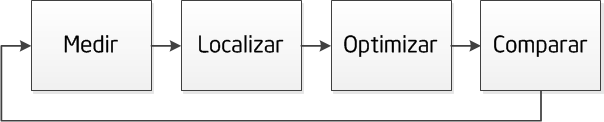
\includegraphics[width=10cm]{cycle.png}
\caption{An\'alisis Iterativo}
\end{center}
\end{figure}

\bigskip

En el caso de tener problemas de desviaci\'on en los resultados medidos, es aconsejable obtener un gran n\'umero de muestras y utilizar
un valor promedio para asegurarse de evitar errores de medici\'on tanto como sea posible. Sin embargo, es siempre preferible aumentar el tama\~no
del problema a resolver, o la definici\'on de los resultados para ejercitar por m\'as tiempo y tener as\'i un resultado m\'as predecible.

\begin{figure}[H]
\begin{center}
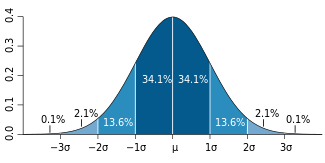
\includegraphics[width=10cm]{deviation.png}
\caption{Desviaci\'on Normal}
\end{center}
\end{figure}

\bigskip

Los resultados deben tambi\'en ser correctamente guardados para evitar
problemas de datos. Si la configuraci\'on del sistema es din\'amica, la reproducci\'on de resultados es compleja, en el caso de no tener una
configuraci\'on de sistema estable en el tiempo, es recomendable siempre
ejecutar una versi\'on optimizada contra una version de referencia en un mismo
sistema de c\'omputo.

\bigskip

Los problemas a identificar inicialmente pueden ser: cuellos de botella,
overhead, problemas de balanceo, contenci\'on o mal uso de recursos
computacionales.

\bigskip

Es muy importante tomar decisiones basadas en datos concretos, ya que en
caso contrario se podr\'ia estar trabajando en lugares donde no se va a obtener
un r\'edito adecuado.

\section{Benchmarks}

Para medir el rendimiento se utilizan pruebas de referencias denominadas
{\em benchmarks}; \'estas pueden ser aplicaciones sint\'eticas constru\'idas
especialmente para ejercitar ciertos recursos computacionales, o pueden ser incluso
aplicaciones del mundo real ejecutadas sobre un conjunto de datos prefijado para
facilitar la comparaci\'on de resultados.

\bigskip

Al tener valores de referencia se pueden caracterizar los sistemas de modo de predecir el rendimiento de una aplicaci\'on.
Los valores a los que se llegan con un {\it benchmark} suelen ser mas practicos y comparables que los teoricos de acuerdo a condiciones ideales der recursos.
Tambi\'en es posible garantizar que el sistema sigue en un mismo estado con el correr del tiempo y los cambios de configuraciones en {\it hardware} o {\it software}.

\bigskip

Las caracter\'isticas deseables en un {\it benchmark} son portabilidad, simplicidad, estabilidad y
reproducci\'on de resultados. Esto permite que sean utilizadas para realizar
mediciones cuantitativas y as\'i realizar comparaciones de optimizaciones o
entre sistemas de c\'omputo diferentes. Tambi\'en se pide que el tiempo de
ejecuci\'on sea razonable y que el tama\~no del problema sea ajustable para
poder seguir siendo \'util con el paso del tiempo y el avance de las
tecnolog\'ias.

\bigskip

A continuaci\'on se introducen algunas de las m\'as utilizadas para c\'omputo
de altas prestaciones, y posteriormente algunos detalles espec\'ificos y ejemplos de sus datos de salida como referencia.

\begin{figure}[H]
  \begin{center}
    \begin{tabular}{|l|l|l|}\hline
      {\bf Benchmark} & {\bf Componente} & {\bf Descripci\'on} \\ \hline
      STREAM & Memoria & Ancho de banda sostenido \\ \hline
      Linpack & Procesador & Operaciones de punto flotante \\ \hline
      IMB & Red & Latencia y ancho de banda de comunicaci\'on \\ \hline
    \end{tabular}
    \caption{Benchmarks}
  \end{center}
  \label{benchmark-list}
\end{figure}

\subsection{STREAM}

STREAM \cite{stream} es un {\it benchmark} sint\'etico a trav\'es de un simple
programa que mide el ancho de banda de memoria sostenido en MB/s y el
rendimiento de computaci\'on relativa de algunos vectores simples de c\'alculo.
Se utiliza para dimensionar el ancho de banda de acceso de escritura o lectura
a la memoria principal del sistema bajo an\'alisis.

\bigskip

Dentro de una misma ejecuci\'on de este {\it benchmark}, se ejercitan diferentes
operaciones en memoria. A continuaci\'on se resumen las operaciones ejercitadas.

\begin{figure}[H]
  \begin{center}
    \begin{tabular}{|l|l|l|}\hline
      {\bf Funci\'on} & {\bf Operaci\'on} & {\bf Descripci\'on} \\ \hline
      copy & $ \forall i $ $ b_{i} = a_{i} $ & Copia simple \\ \hline
      scale & $ \forall i $ $ b_{i} = c \times a_{i} $ & Multiplicaci\'on escalar \\ \hline
      add & $ \forall i $ $ c_{i} = b_{i} + a_{i} $ & Suma directa \\ \hline
      triad & $ \forall i $ $ c_{i} = b_{i} + c \times a_{i} $ & Suma y multiplicaci\'on escalar \\ \hline
    \end{tabular}
    \caption{Operaciones del Benchmark STREAM}
   \end{center}
 \label{stream}
\end{figure}

La salida en pantalla muestra entonces los diferentes tiempos conseguidos y la cantidad de informaci\'on transferida por unidad de tiempo.
Como \'ultimo paso, el programa valida tambi\'en la soluci\'on computada.

\begin{verbatim}
  STREAM version $Revision: 1.2 $
  -------------------------------------------------------------
  This system uses 8 bytes per DOUBLE PRECISION word.
  -------------------------------------------------------------
  Array size = 10000000, Offset = 0
  Total memory required = 228.9 MB.
  Each test is run 10 times, but only the *best* time is used.
  -------------------------------------------------------------
  Function     Rate (MB/s)   Avg time     Min time     Max time
  Copy:        4764.1905       0.0337       0.0336       0.0340
  Scale:       4760.2029       0.0338       0.0336       0.0340
  Add:         4993.8631       0.0488       0.0481       0.0503
  Triad:       5051.5778       0.0488       0.0475       0.0500
  -------------------------------------------------------------
  Solution Validates
\end{verbatim}

\subsection{Linpack}

Linpack \cite{linpack} es un conjunto de subrutinas {\it FORTRAN} que resuelven
problemas de \'algebra lineal como ecuaciones lineales y multiplicaci\'on de
matrices. High Performance Linpack (HPL) \cite{hpl} es una versi\'on portable del {\it benchmark} que incluye
el paquete Linpack pero utilizando sistemas de memoria distribu\'ida.

\bigskip

Existe cierta controversia de que no es una buena forma de ejercitar un
sistema de c\'omputo distribu\'ido ya que no implica uso significativo de la
red, s\'olo procesamiento intensivo de aritm\'etica de punto flotante
sobre la jerarqu\'ia local de memoria.

\bigskip

Sin embargo, este benchmark es utilizado mundialmente para la comparaci\'on de la
velocidad de las supercomputadoras en el ranking TOP500. 
Un gr\'afico del TOP500 de los \'ultimos a\~nos demuestra claramente la
tendencia en crecimiento de rendimiento; tambi\'en la relaci\'on entre el primero, el último y la suma de todos los sistemas en la lista.

\begin{figure}[H]
\begin{center}
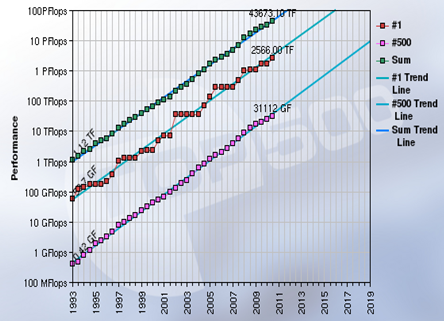
\includegraphics[width=10cm]{top500.png}
\caption{Indicadores Hist\'oricos del Top500}
\end{center}
\end{figure}

Este {\it benchmark} requiere conocimiento avanzado para una correcta configuraci\'on,
por ejemplo el tama\~no de bloque que se va a utilizar para la distribuci\'on de trabajo
debe estar directamente relacionado con el tama\~no del {\it cache} de memoria del procesador.

\bigskip

La salida en pantalla resume entonces los datos de entrada y los resultados conseguidos.
Como \'ultimo paso el programa valida que los resultados sean correctos.

\begin{verbatim}
=================================================================
HPLinpack 2.0 - High-Performance Linpack benchmark - Sep 10, 2008
Written by A. Petitet and R. Clint Whaley
============================================================
An explanation of the input/output parameters follows:
T/V    : Wall time / encoded variant.
N      : The order of the coefficient matrix A.
NB     : The partitioning blocking factor.
P      : The number of process rows.
Q      : The number of process columns.
Time   : Time in seconds to solve the linear system.
Gflops : Rate of execution for solving the linear system.

The following parameter values will be used:
N      :   28888
NB     :     168
PMAP   : Row-major process mapping
P      :       4
Q      :       4
PFACT  :   Right
NBMIN  :       4
NDIV   :       2
RFACT  :   Crout
BCAST  :  1ringM
DEPTH  :       0
SWAP   : Mix (threshold = 64)
L1     : transposed form
U      : transposed form
EQUIL  : yes
ALIGN  : 8 double precision words
-------------------------------------------------------------------------------
- The matrix A is randomly generated for each test.
- The relative machine precision (eps) is taken to be 1.110223e-16
- Computational tests pass if scaled residuals are less than 16.0

Column=000168 Fraction=0.005 Mflops=133122.97
...
Column=025872 Fraction=0.895 Mflops=98107.60
==========================================================================
T/V                N   NB   P    Q             Time                 Gflops
WR01C2R4       28888  168   4    4           165.83              9.693e+01
--------------------------------------------------------------------------
||Ax-b||_oo/(eps*(||A||_oo*||x||_oo+||b||_oo)*N) = 0.0043035 ...... PASSED
==========================================================================
Finished      1 tests with the following results:
1 tests completed and passed residual checks,
0 tests completed and failed residual checks,
0 tests skipped because of illegal input values.
\end{verbatim}

\subsection{Intel MPI Benchmarks}

Es un conjunto de {\it benchmarks} cuyo objetivo es ejercitar las funciones
m\'as importantes del estandar para librer\'ias de paso de mensajes (MPI, por sus siglas en ingl\'es) \cite{mpi}.
El m\'as conocido es el popular ping-pong, el cual ejercita la transmisi\'on de mensajes ida y vuelta entre dos nodos de
c\'omputo con diferentes tama\~nos de mensajes. 

\bigskip

Este {\it benchmark} es uno de los m\'as utilizados por su simpleza, 
en particular para comprobar que los dispositivos de red est\'en configurados adecuadamente para c\'omputo
de altas prestaciones.

\bigskip

Para obtener el m\'aximo ancho de banda disponible, se ejercita la comunicaci\'on a trav\'es de mensajes con datos grandes.
Para obtener la m\'inima latencia, se ejercita la comunicaci\'on con mensajes vac\'ios, es decir transmitiendo mensajes sin datos.

\begin{verbatim}
# Intel (R) MPI Benchmark Suite V3.1, MPI-1 part
# Date                  : Wed Mar  3 10:45:16 2010
# Machine               : x86_64
# System                : Linux
# Release               : 2.6.16.46-0.12-smp
# Version               : #1 SMP Thu May 17 14:00:09 UTC 2007
# MPI Version           : 2.0
# MPI Thread Environment: MPI_THREAD_SINGLE
# Calling sequence was: ../IMB-MPI1 pingpong
# Minimum message length in bytes:   0
# Maximum message length in bytes:   4194304
#
# MPI_Datatype                   :   MPI_BYTE
# MPI_Datatype for reductions    :   MPI_FLOAT
# MPI_Op                         :   MPI_SUM
#
# List of Benchmarks to run: PingPong
#---------------------------------------------------
# Benchmarking PingPong
# #processes = 2
#---------------------------------------------------
#bytes     #repetitions  t[usec]     Mbytes/sec
0              1000           17.13        0.00
1              1000           17.89        0.05
2              1000           17.82        0.11
4              1000           17.95        0.21
...
1048576    40              8993.23    111.19
2097152    20              17919.20  111.61
4194304    10              35766.45  111.84
\end{verbatim}

\subsection{HPCC}

El {\it benchmark} HPC Challenge \cite{hpcc} (HPCC) est\'a compuesto internamente por un conjunto de
varios {\it benchmarks}, entre ellos STREAM, HPL, Ping Pong, Transformadas de {\it Fourier}
y otros.

\bigskip

Este benchmark muestra diferentes resultados que son representativos
y puestos en consideraci\'on de acuerdo al tipo de aplicaci\'on en discusi\'on.
La mejor m\'aquina depende de la aplicaci\'on a ejecutar, ya que algunas aplicaciones
necesitan mejor ancho de banda de memoria, mejor canales de comunicaci\'on, o
la mayor capacidad de c\'omputo posible.

\bigskip

Una analog\'ia interesante para entender como el {\it benchmark} se relaciona a diferentes n\'ucleos de c\'omputo
se muestra a continuaci\'on.

\bigskip

\begin{figure}[H]
\begin{center}
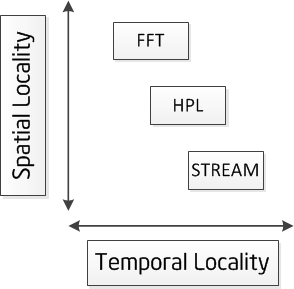
\includegraphics[width=10cm]{locality.png}
\caption{Localidad}
\end{center}
\end{figure}

\bigskip

Para una mejor comparaci\'on de resultados de HPCC, se utilizan diagramas denominados {\it kiviats}.

\begin{figure}[H]
\begin{center}
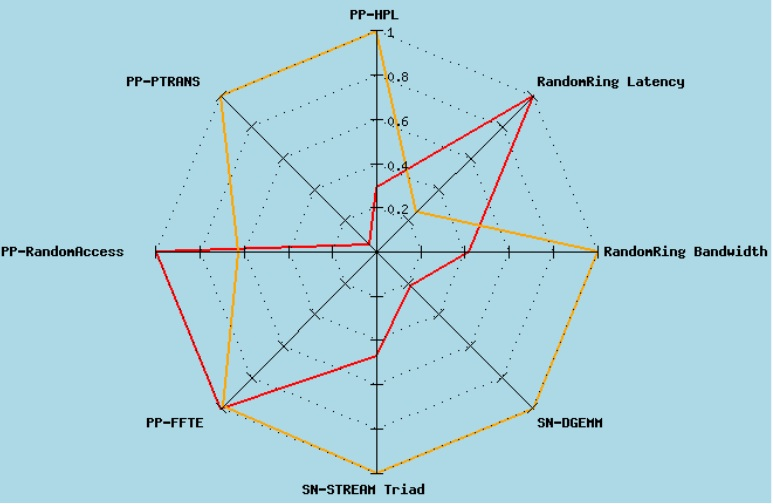
\includegraphics[width=10cm]{kiviat.png}
\caption{Diagrama Kiviat}
\end{center}
\end{figure}

Un ejemplo de la salida que se muestra durante la ejecuci\'on se muestra a continuaci\'on.

\begin{verbatim}
This is the DARPA/DOE HPC Challenge Benchmark version 1.2.0 October 2003
Produced by Jack Dongarra and Piotr Luszczek
Innovative Computing Laboratory
University of Tennessee Knoxville and Oak Ridge National Laboratory
See the source files for authors of specific codes.
Begin of Summary section.
\end{verbatim}

\begin{minipage}[b]{0.5\linewidth}
\begin{verbatim}
VersionMajor=1
VersionMinor=2
LANG=C
Success=1
CommWorldProcs=3
MPI_Wtick=1.000000e-06
HPL_Tflops=0.0674008
HPL_time=26.3165
HPL_eps=1.11022e-16
HPL_N=13856
HPL_NB=64
HPL_nprow=1
HPL_npcol=3
HPL_depth=2
HPL_nbdiv=2
HPL_nbmin=8
HPL_cpfact=C
HPL_crfact=R
HPL_ctop=1
HPL_order=R
dweps=1.110223e-16
sweps=5.960464e-08
HPLMaxProcs=3
HPLMinProcs=3
DGEMM_N=4618
StarDGEMM_Gflops=68.9053
SingleDGEMM_Gflops=70.2692
PTRANS_GBs=0.794254
PTRANS_time=0.479293
PTRANS_residual=0
PTRANS_n=6928
PTRANS_nb=64
PTRANS_nprow=1
PTRANS_npcol=3
MPIRandomAccess_N=134217728
MPIRandomAccess_time=30.4475
MPIRandomAccess_CheckTime=14.0705
MPIRandomAccess_Errors=0
\end{verbatim}
\end{minipage}
\hspace{0.5cm}
\begin{minipage}[b]{0.5\linewidth}
\begin{verbatim}
MPIRandomAccess_ErrorsFraction=0
MPIRandomAccess_ExeUpdates=536870912
MPIRandomAccess_GUPs=0.0176327
MPIRandomAccess_TimeBound=-1
MPIRandomAccess_Algorithm=0
RandomAccess_N=33554432
StarRandomAccess_GUPs=0.0186362
SingleRandomAccess_GUPs=0.0184568
STREAM_VectorSize=21332081
STREAM_Threads=8
StarSTREAM_Copy=4.34705
StarSTREAM_Scale=3.24366
StarSTREAM_Add=3.41196
StarSTREAM_Triad=3.46198
SingleSTREAM_Copy=4.53628
SingleSTREAM_Scale=3.38984
SingleSTREAM_Add=3.59073
SingleSTREAM_Triad=3.65083
FFT_N=8388608
StarFFT_Gflops=2.17339
SingleFFT_Gflops=2.26806
MPIFFT_N=8388608
MPIFFT_Gflops=1.7043
MPIFFT_maxErr=1.77722e-15
MPIFFT_Procs=2
MaxPingPongLatency_usec=5.37932
RandomlyOrderedRingLatency_usec=5.70686
MinPingPongBandwidth_GBytes=0.675574
NaturallyOrderedRingBandwidth_GBytes=0.531278
RandomlyOrderedRingBandwidth_GBytes=0.529161
MinPingPongLatency_usec=5.24521
AvgPingPongLatency_usec=5.30978
MaxPingPongBandwidth_GBytes=0.682139
AvgPingPongBandwidth_GBytes=0.678212
NaturallyOrderedRingLatency_usec=5.79357
FFTEnblk=16
FFTEnp=8
FFTEl2size=1048576
\end{verbatim}
\end{minipage}

\begin{verbatim}
End of Summary section.
End of HPC Challenge tests.
\end{verbatim}

\section{Teor\'ia}

Una vez obtenida una implementaci\'on eficiente, la \'unica alternativa para mejorar el rendimiento es explotar el paralelismo que
ofrecen los sistemas de c\'omputo. Este paralelismo se puede explotar a diferentes niveles, desde instrucciones que ejecutan una misma instruccion a varios
datos a la vez, pasando por la utilizacion varias unidades de computo en el mismo sistema hasta la utilizacion de unidades de computo en diferentes sistemas.

\bigskip

El c\'alculo de las mejoras posibles de rendimiento, como priorizarlas y su l\'imite m\'aximo es una tarea no trivial.
Para ello existen algunas leyes frecuentemente utilizadas durante el an\'alisis de rendimiento.

\subsection{Ley de {\it Amdahl}}

 La ley de {\it Amdahl} \cite{amdahl} dimensiona la mejora que puede obtenerse en un sistema de acuerdo a las mejoras logradas en sus
componentes. Nos ayuda a establecer un l\'imite m\'aximo de mejora y a conocer de antemano cuales pueden ser los resultados de mejora.

\bigskip

La mejora de un programa utilizando procesamiento multiple en c\'omputo paralelo est\'a limitado por el tiempo necesario para completar su fracci\'on serial o secuencial. Frecuentemente el paralelismo solo afecta notariamente cuando es utilizado en un peque\~no n\'umero de procesadores, o cuando se aplica a problemas altamente escalables (embarrassingly parallel problems). Una vez paralelizado un programa, los esfuerzos suelen ser enfocados en como minimizar
la parte secuencial, algunas veces haciendo m\'as trabajo redundante en paralelo.

\bigskip

La ley de amdahl puede ser entonces modelada de la siguiente forma:

\begin{eqnarray}
max speedup = \frac{1}{(1-P) + \frac{P}{N}}
\end{eqnarray}

donde $ P $ es el porcentaje de trabajo paralelizable ($ 1-P $ es entonces el trabajo en serie o secuencial), $ N $ es la cantidad de unidades de c\'omputo utilizadas.

\bigskip

Suponiendo que una aplicaci\'on requiere de un trabajo serial más un trabajo paralelizable; esta ley nos deja estimar la m\'axima ganancia posible
de modo que incluso teniendo infinitas unidades de c\'omputo la ganancia esta limitada como se muestra a continuaci\'on. Incluso en el caso de tener varias
componentes aisladas en la parte paralela, esta ley nos ayuda a identificar el impacto al mejorar cada una de las partes.

\begin{figure}[H]
\begin{center}
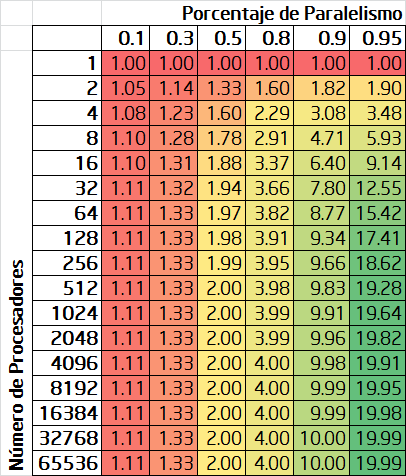
\includegraphics[width=5cm]{amdahl.png}
\caption{Mejora M\'axima}
\end{center}
\end{figure}

La tabla anterior nos muestra que no importa la cantidad de unidades de procesamiento que sean utilizadas, en el caso de solo tener un 10\% de paralelismo
en una aplicacion, la mejora nunca va a superar 1.10x la original. En el caso de tener un 95\%, la mejora nunca va a ser mejor a 20x. Es poco frecuente encontrar aplicaciones que sean altamente paralelizables, la mayoria solo muestra beneficios relevantes al ser escalada hasta 1024 procesadores.

\subsection{Ley de {\it Gustafson}}

Desde un punto de vista m\'as general, la ley de {\it Gustafson}
\cite{gustafson} establece que las aplicaciones que manejan problemas
repetitivos con conjuntos de datos similares pueden ser f\'acilmente
paralelizadas. En comparaci\'on, la ley anterior no escala el tama\~no o
resoluci\'on de problema cuando se incrementa la potencia de c\'alculo, es
decir con un tama\~no de problema fijo. 

\bigskip

Al aplicar esta ley obtenemos que un problema con datos grandes o repetitivos en cantidades grandes puede ser
eficientemente paralelizable. Nos es \'util para determinar el tama\~no de problema a utilizar cuando los recursos de c\'omputo son incrementados.
En el mismo tiempo de ejecucion, el programa resuelve entonces problemas m\'as grandes.

\begin{eqnarray}
speedup(P) = P - \alpha . ( P - 1)
\end{eqnarray}

donde $ P $ es el n\'umero de unidades de c\'omputo y $ \alpha $ el porcentaje de trabajo paralelizable.

\begin{figure}[H]
\begin{center}
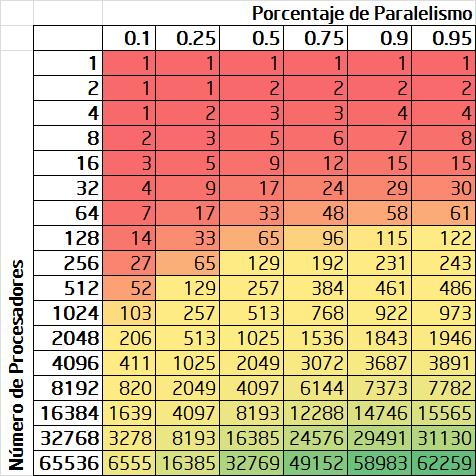
\includegraphics[width=5cm]{gustafson.png}
\caption{Tama\~no de Datos de Entrada}
\end{center}
\end{figure}

Similarmente al cuadro anterior, podemos deducir que en el caso de un programa con s\'olo 10\% de paralelismo, al incrementar los recursos 64x s\'olo podemos incrementar el tama\~no del problema 7x. Sin embargo nos recomienda incrementar 61x en el caso de tener 95\% de paralelismo.

\subsection{M\'etrica de {\it Karp-Flatt}}

Esta m\'etrica es utilizada para medir el grado de paralelismo de una aplicaci\'on \cite{karp-flatt}.
Esta m\'etrica nos permite rapidamente estimar la mejora posible al aplicar un alto nivel de paralelismo.

\bigskip

Given a parallel computation exhibiting speedup ψ on p processors, where p > 1, the experimentally determined serial fraction e is defined to be the Karp–Flatt Metric viz: The less the value of e the better the parallelization.

For a problem of fixed size, the efficiency of a parallel computation typically decreases as the number of processors increases. By using the serial fraction obtained experimentally using the Karp–Flatt metric, we can determine if the efficiency decrease is due to limited opportunities of parallelism or increases in algorithmic or architectural overhead.

\begin{eqnarray}
 e = \frac{\frac{1}{\psi} - \frac{1}{p}}{1 - \frac{1}{p}} 
\end{eqnarray}

\section{Patrones de Dise\~no}

Entre los patrones de dise\~no m\'as discutidos se encuentran: master/worker,
pipeline, work-stealing. En el dise\~no master/worker, un proceso dirige el
trabajo de los dem\'as. En pipeline el trabajo se divide en etapas
independendientes. En work-stealing los trabajadores obtienen el trabajo desde
un conjunto en com\'un.

\begin{figure}[H]
\begin{center}
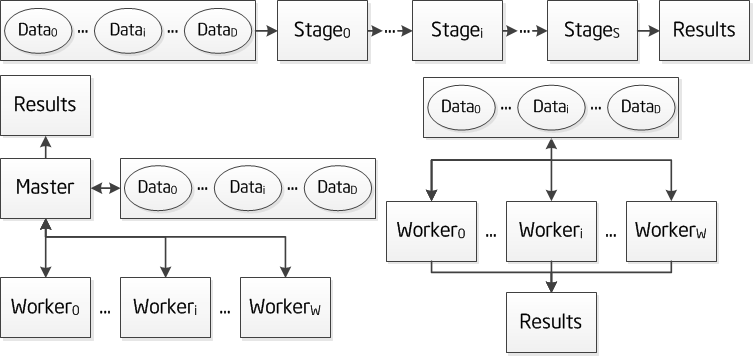
\includegraphics[width=10cm]{patterns.png}
\caption{Patrones}
\end{center}
\end{figure}

\subsection{Pipeline}

Este dise\~no establece una divisi\'on del trabajo en etapas aisladas.

Cada etapa puede ser computada al mismo tiempo, por lo que las unidades de trabajo que transitan las etapas pueden ser solapadas entre si.
Aunque la cantidad de trabajo es el mismo, el solapamiento permite completar mas unidades de trabajo en N etapas al momento N+i con i=1.

\subsection{Master/Worker}

Maestro/Trabajador.

Balanceo de carga.

\subsection{Work-Stealing}

Robo de Trabajo.

Balanceo de carga automatico, sin importan si son unidades de c\'omputo heterogeneo.

\chapter{Herramientas}

Este cap\'itulo revisa las herramientas disponibles para soporte de an\'alisis
de rendimiento de aplicaciones.

\section{Taxonom\'ia}

Existen diferentes alternativas sobre el modo de extraer informaci\'on de
caracter\'isticas relacionadas con el rendimiento de una aplicaci\'on.
Estos m\'etodos pueden clasificarse como din\'amico o est\'atico.
Tambi\'en pueden clasificarse como aplicables en tiempo de compilaci\'on o
tiempo de ejecuci\'on.

% TBD: insert nice chart here, get inspired from wikipedia clasifications

\section{gprof}

Esta herramienta extrae el perfil din\'amico de una aplicaci\'on, en tiempo
de ejecuci\'on. Se instrumenta la aplicacion con una opci\'on espec\'ifica que
incluye informacion de uso de las diferentes partes del programa y los
recursos del sistema como procesador y memoria.

\bigskip

La aplicaci\'on debe ejecutarse con un conjunto de datos dado. El conjunto de
datos debe ser representativo y debe tambi\'en ejercitar la aplicaci\'on por
una cantidad de tiempo suficiente como para intensificar el uso de los
recursos. Los datos del perfil de una ejecuci\'on son luegos obtenidos en la
forma de un archivo de datos, luego se procede a procesar los datos acumulados
con un analizador respectivo.

\bigskip

Provee un perfil plano que consiste en una simple lista de las funciones
ejecutadas ordenadas por la cantidad acumulada de tiempo utilizado.
Tambi\'en provee el gr\'afico de llamadas anidadas, que muestra el tiempo
utilizado por cada funci\'on en llamadas sucesivas. Las funciones recursivas
son manejadas de manera especial ya que imposibilitan el armado de relaciones
de dependencias.

\subsection{Perfil de Ejecuci\'on}

El perfil de ejecuci\'on muestra el tiempo individual y el tiempo acumulado en segundos
de cada l\'inea de c\'odigo de la aplicaci\'on.

{\tt time, cumulative seconds, self seconds, calls, self ms/call,
  total ms/call, name}

\subsection{Gr\'afico de llamadas}

index, \% time, self, children, called, name

La herramienta tambi\'en muestra un cuadro de las llamadas entre funciones realizadas por el programa.
Esto permite visualizar el esquema de dependencias durante la ejecuci\'on.

\subsection{Comportamiento}

precisi\'on estad\'istica. muestreo. incompatibilidades.

\subsection{Ejemplos}

\section{oprofile}

\subsection{Introducci\'on}

historia. resumen. caracter\'isticas. 

\subsection{Procedimiento}

ejecutar el profiler. ejecutar la aplicaci\'on. generar el resumen.

No se necesita el c\'odigo. C\'odigo anotado si hay s\'imbolos de depuraci\'on o
{\it debugging}.

componentes del sistema.

contadores de performance.

costo adicional. overhead.

\subsection{Contadores de Rendimiento}

Los registros de {\it hardware} implementando contadores m\'as utilizados son los
siguientes:

\begin{enumerate}
\item total processor cycles
\item total instructions
\item cycles stalled waiting for memory accesses
\item floating point divide instructions
\item L1 cache misses
\item floating point instructions
\item load instructions
\item store instructions
\end{enumerate}

\subsection{Ejemplos}

\chapter{Procedimiento de An\'alisis}

\section{Proceso}

Modificaciones controladas.

\bigskip

Medir. Analizar. Optimizar. Comparar.

\section{Actividades}

\subsection{Medici\'on}

Como medir? Benchmark repetible. Baja Desviacion. No muy rapido pero por unos
minutos. Si hay mucha deviacion se debe repetir la medicion muchas veces y
tomar el promedio.

\subsection{An\'alisis}

Como analizar? Pareto. State-of-the-art. Librerias para el mismo problema.
Como dibujar un pareto? Como se entiende un pareto?

Un gr\'afico de Pareto incluye tanto un diagrama de barras como uno de l\'ineas, ambos superpuestos.
Los valores individuales son representados en orden descendiente en las barras, y el valor acumulado del porcentaje total es representado con una l\'inea.

Esto permite identificar r\'apidamente el lugar a optimizar. El componente, archivo, funci\'on, c\'odigo, instrucci\'on.

\subsection{Optimizaci\'on}

Como optimizar? Librerias. Dependencias. Paralelizar.

\subsection{Comparaci\'on}

C\'omo comparar? Antes/Despues. Repeticiones. Para utilizar informaci\'on
hist\'orica es preciso garantizar que el sistema siendo ejercitado es el mismo. Por ello es preferible ser cautos y ejecutar las dos versiones conjuntamente
al momento de realizar las pruebas. 

\chapter{Modelo}

Este cap\'itulo propone la utilizaci\'on de un modelo por etapas para el desarrollo de aplicaciones de alto rendimiento.
Se introduce la propuesta y la justificaci\'on de su utilizaci\'on para un mejor an\'alisis de rendimiento.

\section{Definici\'on}

Modelo por etapas. F\'acil de identificar donde realizar optimizaciones y la ganancia esperada.

% TBD: insertar dibujo del modelo por etapas

Este patr\'on de dise\~no tiene grandes beneficios adem\'as de su simplicidad. Checkpointing. Serial. Paralelo. Pareto.

Visualizaci\'on directa.

\section{An\'alisis}

 El c\'alculo de las leyes de amdalah y dem\'as es directo.

\subsection{F\'ormulas}

% TBD: insertar formulas asumiendo un modelo por etapas

\bigskip

F\'ormulas de tiempo de ejecuci\'on. amdalah.

\chapter{Casos de Estudio}

Este cap\'itulo aplica el modelo propuesto en el cap\'itulo anterior. Varios ejemplos no triviales de aplicaciones de altas prestaciones son implementados
y analizados utilizando los benchmarks y herramientas anteriormente presentadas.

\section{Multiplicaci\'on de Matrices}

La multiplicaci\'on de matrices es una operaci\'on fundamental en m\'ultiples
campos de aplicaci\'on cient\'ifica como la resoluci\'on de ecuaciones
lineales y la representaci\'on de grafos y espacios dimensionales. Por ello
existe abundante material sobre el tema.

\begin{verbatim}
for (i = 0; i < n; i++)
  for (j = 0; j < n; j++)
    for (k = 0; k < n; k++)
      c[i * n + j] += 
        a[i * n + k] * b[k * n + j];
\end{verbatim}

Diferentes alternativas de implementaci\'on son discutidas en
\cite{mm-matrixmultiplicationtool}.

\bigskip

El c\'odigo fuente de una implementaci\'on simplista se encuentra adjuntado en
el ap\'endice. Al aplicar las herramientas vistas previamente se identifica
claramente que la multiplicaci\'on de los elementos de la matriz consume el
mayor tiempo de c\'omputo.

\bigskip



\bigskip

A continuaci\'on se muestra una comparaci\'on de diferentes m\'etodos, se
demuestra claramente con este ejercicio la sofisticaci\'on de librer\'ias
contra m\'etodos artesanales de optimizaci\'on.

\section{Distribuci\'on de Calor en Dos Dimensiones}

\begin{verbatim}
  for (j = 1; j < matrix_height - 1; j++) {
    for (i = 1; i < grid_length - 1; i++) {
      
      matrix[j * grid_length + i] = 
                     0.25 * (tmp[j * grid_length + i - 1]
                  + tmp[j * grid_length + i + 1]
                  + tmp[(j - 1) * grid_length + i]
                  + tmp[(j + 1) * grid_length + i]);

      diff = matrix[pos(i,j)] - tmp[pos(i,j)];

      if (error < diff) {
         error = diff;
      }
    }
  }
\end{verbatim}

La salida del c\'alculo puede graficarse f\'acilmente con {\it gnuplot}.

\begin{figure}[H]
\begin{center}
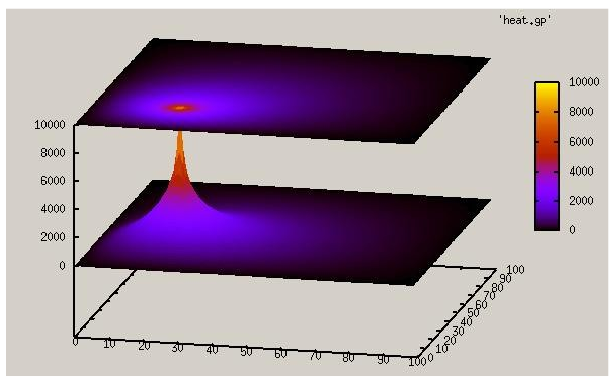
\includegraphics[width=10cm]{heat2d.png}
\caption{heat2d}
\end{center}
\end{figure}

\section{Problema de las Ocho Reinas}

El dilema trata en el problema de posicionar en un tablero de ajedrez ocho
reinas sin que alguna amenace a las dem\'as. Una reina amenaza a cualquier otra
pieza en el tablero que este en la mismo diagonal, fila o columna.

\bigskip

Este problema suele resolverse utilizando recursi\'on.

\begin{verbatim}
int columns = 8;
int column = 0;
for (column = 0; column < columns; column++)
   queen();

void queen() {
   queen();
}
\end{verbatim}

\section{Transformadas de {\it Fourier}}

Una transformada de {\it Fourier} \cite{fourier} transforma una se\~nal
digitalizada en una representaci\'on matem\'atica de las frecuencias que la
componen. Su aplicaci\'on principal se da en problemas relacionados con el
movimiento de ondas como en la \'optica y electromagnetismo.

\bigskip

El c\'odigo fuente de una implementaci\'on simplista se encuentra adjuntado en
el ap\'endice. Al aplicar las herramientas vistas previamente se identifica
claramente que la evaluaci\'on de derivadas parciales consume el mayor tiempo
de c\'omputo.

\bigskip

A continuaci\'on se muestra una comparaci\'on de diferentes m\'etodos, se
demuestra claramente con este ejercicio la sofisticaci\'on de librer\'ias
contra m\'etodos artesanales de optimizaci\'on. La siguiente es la versi\'on
cl\'asica de una implementacion directa utilizando el algoritmo de
{\it Cooley-Tukey}.

\begin{verbatim}
int i, k;
float arg, sign = -1.0;

for (i = 0; i <= length/2; i++) {
    cosine[i] = sine[i] = 0.0;
    for (k = 0; k < length; k++) {
        arg = 2.0 * i * M_PI * k / length;
        sine[i] += input[k] * sign * sin(arg);
        cos[i] += input[k] * cos(arg);
    }
}
\end{verbatim}

\begin{verbatim}
int i;

for (i = 0; i <= length / 2; i++) {
    frequency[i] = 1.0 * i * rate / length;
    magnitude[i] =
        20.0 *
        log10( 2.0 * sqrt(sine[i] * sine[i] + cosine[i] * cosine[i]) /
        length);

    phase[i] = 180.0 * atan2(sine[i], cosine[i]) / M_PI - 90.0;
}
\end{verbatim}

Una implementaci\'on m\'as eficiente es la denominada {\it Fast Fourier Transform}.
Un algoritmo a\'un m\'as eficiente es el denominado {\it Goertzel}.

\bigskip

Este caso de aplicacion no demuestra como al conocer el algoritmo implementado se
facilita la tarea de buscar algoritmos optimizados para cada caso en particular.

\chapter{Conclusiones}

Este trabajo aporta el estado del arte del an\'alisis de rendimiento en
aplicaciones de c\'omputo de altas prestaciones. Discute, clasifica y detalla
diferentes opciones en herramientas de soporte. Se demuestra su aplicaci\'on
en varios problemas simples pero suficientemente interesantes. Propone un
proceso y un modelo simple de implementaci\'on para dimensionar las
optimizaciones posibles.

\bigskip

La optimizaci\'on del rendimiento de una aplicaci\'on es algo no trivial, requiere de mucha
disciplina y del manejo de datos que identifiquen las partes a mejorar fehacientemente.
Existen diferentes niveles de abstracci\'on en los cuales una aplicaci\'on puede ser analizada con el fin
de encontrar puntos de mejora. 

\bigskip

Es preciso realizar un an\'alisis del comportamiento y del uso de los recursos antes de
empezar a optimizar una aplicaci\'on. Muchas veces las mejoras no son significativas si no
son realizadas en el lugar correcto.

\bigskip

El utilizar un mismo modelo para implementar las aplicaciones abre muchas puertas para
la automatizaci\'on, comparaci\'on y estudio de t\'ecnicas de optimizaci\'on que no pueden
ser siempre aplicadas sin reestructurar las aplicaciones.

\chapter{Trabajo Futuro}

\section{Infrastructura de Soporte para An\'alisis}

Este trabajo fue realizado como un primer paso a una implementaci\'on pr\'actica del m\'etodo propuesto,
incluyendo soporte autom\'atico para al utilizaci\'on de las herramientas y la generaci\'on integrada de
reportes de an\'alisis de rendimiento.

\section{Herramientas Adicionales de Soporte}

La implementaci\'on de nuevas tecnolog\'ias para el an\'alisis de rendimiento
es incesante y continua, los siguientes proyectos est\'an ampliamente
relacionados con este estudio.

\begin{itemize}
\item Proyecto A: descripci\'on del proyecto A.
\item Proyecto B: descripci\'on del proyecto B.
\item Proyecto C: descripci\'on del proyecto C.
\end{itemize}

\section{Aplicaci\'on en el Mundo Real}

La utilizaci\'on de estas ideas en una aplicaci\'on del mundo real es materia
pendiente, otra posibilidad es reimplementar desde cero alguna aplicaci\'on
cient\'ifica en colaboraci\'on con alg\'un grupo de investigaci\'on y realizar
varios ciclos de optimizaci\'on.

\bigskip

Trabajo en conjunto con un alg\'un grupo de investigaci\'on cient\'ifica,
realizando an\'alisis de rendimiento de aplicaciones ya existentes utilizadas
para publicaci\'on de resultados de modelado o simulaci\'on.

\begin{thebibliography}{9}

\bibitem{mm-matrixmultiplicationtool}
  A. More,
  \emph{A Case Study on High Performance Matrix Multiplication},
  {\tt http://code.google.com/p/mm-matrixmultiplicationtool},
  2008.

\bibitem{parallel-programming}
  Paul E. McKenney,
  \emph{Is Parallel Programming Hard, And, If So, What Can You Do About It?},
  January, 2011.

\bibitem{fourier}
  J. B. Joseph Fourier, \emph{Th\'eorie Analytique de la Chaleur}, Paris, 1822.

\bibitem{beowulf}
  T. Sterling, D. Savarese, D. J. Becker, J. E. Dorband, U. A. Ranawake,
  and C. V. Packer,
  \emph{Beowulf: A parallel workstation for scientific computation},
  1995.

\bibitem{mpi}
  Message Passing Interface Forum,
  \emph{MPI: A Message-Passing Interface Standard},
  2.2,
  2009.

\bibitem{openmp}
  OpenMP Architecture Review Board,
  \emph{OpenMP Application Program Interface}.
  3.0,
  2008.

\bibitem{tinetti}
  Fernando G Tinetti,
  \emph{C\'omputo Paralelo en Redes Locales de Computadoras},
  2004.

\bibitem{gprof}
  Susan L. Graham,  Peter B. Kessler,  Marshall K. McKusick,
  \emph{gprof: A Call Graph Execution Profiler},
  1982.
  
\bibitem{oprofile}
  J. Levon,
  \emph{oprofile: hardware profiler for Linux systems},
       {\tt http://oprofile.sourceforge.net}.
  
\bibitem{hennessy-patterson}
  John. L. Hennesy, David A. Patterson,
  \emph{Computer Architecture: A Quantitative Approach, 3rd Edition},
  2002.

\bibitem{intel}
  Intel Press,
  \emph{Intel64 and IA-32 Architectures Software Developer's Manual - Volume
    3B: System Programming Guide, Part 2},
  March 2010.

\bibitem{what}
  Ulrich Deeper,
  \emph{What Every Programmer Should Know About Memory},
  November 2007.

\bibitem{patterns}
  G. Mattson, B.A. Sanders and B.L. Massingill, 
  \emph{Patterns for Parallel Programming, Addison-Wesley},
  2004.
  
\bibitem{automatic-performance-analysis}
  T. Margalef, J. Jorba, O. Morajko, A. Morajko, E. Luque,
  \emph{Different approaches to automatic performance analysis of distributed
    applications},
  2004.
  
\bibitem{capturing-performance-knowledge}
  K. Huck, O. Hernandez, V. Bui, S. Chandrasekaran, B. Chapman, A. Malony,
  L McInnes, B. Norris,
  \emph{Capturing performance knowledge for automated analysis},
  2008.
  
\bibitem{automatic-openmp-mpi-analysis}
  F. Wolf, B. Mohr,
  \emph{Automatic performance analysis of hybrid MPI/OpenMP applications},
  2003.
  
\bibitem{intro-software-performance}
  C. Smith,
  \emph{Introduction to software performance engineering: origins and
    outstanding problems},
  2007.

\bibitem{future-software-performance}
  M. Woodside, G. Franks, D. Petriu,
  \emph{The Future of Software Performance Engineering},
  2007.

\bibitem{critical-overview}
  J. Browne,
  \emph{A critical overview of computer performance evaluation},
  1976.

\bibitem{hpctoolkit}
  Rice University,
  \emph{HPC Toolkit}, {\tt http://hpctoolkit.org}.
       
\bibitem{papi}
  University of Tennessee,
  \emph{Performance Application Programming Interface},
       {\tt http://icl.cs.utk.edu/papi}.
       
\bibitem{amdahl}
  G. M. Amdahl,
  \emph{Validity of single-processor approach to achieving large-scale
    computing capability},
  Proceedings of AFIPS Conference, Reston, VA. 1967. pp. 483-485.
  
\bibitem{twelve-ways}
  D. Bailey, \emph{Twelve Ways to Fool the Masses When Giving Performance
    Results on Parallel Computers},
  RNR Technical Report, RNR-90-020, NASA Ames Research Center, 1991.
  
\bibitem{gustafson}
  J. L. Gustafson,
  \emph{Reevaluating Amdahl's Law}, CACM, 31(5), 1988. pp. 532-533.
  
\bibitem{karp-flatt}
  A. H. Karp and H. P. Flatt,
  \emph{Measuring Parallel Processor Performance},
  Communication of the ACM Volume 33 Number 5, May 1990.
  
\bibitem{myth}
  {Lee, Victor W. and Kim, Changkyu and Chhugani, Jatin and Deisher, Michael
    and Kim, Daehyun and Nguyen, Anthony D. and Satish, Nadathur and
    Smelyanskiy, Mikhail and Chennupaty}, Srinivas, and Hammarlund, Per and
  Singhal, Ronak and Dubey, Pradeep,
  \emph{Debunking the 100X GPU vs. CPU myth: an evaluation of throughput
    computing on CPU and GPU},
  2010.
  
\bibitem{stream}
  John D. McCalpin,
  \emph{A Survey of Memory Bandwidth and Machine Balance in Current High
    Performance Computers},
  1995.
  
\bibitem{counters}
  Dong H. Ahn and Jeffrey S. Vetter,
  \emph{Scalable Analysis Techniques for Microprocessor Performance Counter
    Metrics},
  2002.
  
\bibitem{linpack}
  J. Dongarra, J. Bunch, C. Moler and G. W. Stewart, 
  \emph{LINPACK Users Guide},
  1979.
  
\bibitem{hpl}
  A. Petitet, R. C. Whaley, J. Dongarra and A. Cleary, 
  \emph{HPL - A Portable Implementation of the High-Performance Linpack
    Benchmark for Distributed-Memory Computers}, {\tt http://www.netlib.org/benchmark/hpl}
  2008.

\bibitem{hpcc}
  Dongarra, J., Luszczek, P.,
  \emph{Introduction to the HPC Challenge Benchmark Suite}, ICL Technical Report,
  2005.  
  
\bibitem{gsl}
  Free Software Foundation (FSF), \emph{GNU Scientific Library (GSL)},
  {\tt http://www.gnu.org/software/gsl}.

\end{thebibliography}

\end{document}
